\begin{document}

\emph{Tumori benigni cartilaginei}

Encondroma solitario

Neoplasia caratterizzata dalla formazione di cartilagine matura
all'interno dell'osso e di solito localizzata in corrispondenza delle
\textbf{metafisi} delle ossa lunghe.

È generalmente \textbf{asintomatica} ed è più frequente tra i 15 e 50
anni.

La diagnosi è una diagnosi radiografica occasionale.

Come primo segno l'encondroma può dare delle \emph{fratture patologiche}
soprattutto a livello delle mani, dei metacarpi, delle falangi.

Dal punto di vista \textbf{radiografico} abbiamo delle zone di lisi,
ossia delle zone osteolitiche con dei punti radio opachi all'interno.

Il \textbf{trattamento} di solito può essere nullo, ma nel momento in
cui la neoplasia provoca fastidio o si associa a delle fratture
patologiche si può procedere con courrettage chirurghico (ossia una
pulizia del focolaio encondromatoso) e poi borraggio (ossia si va a
mettere in questo ``buco'' osso autologo o innesto osseo da cadavere).

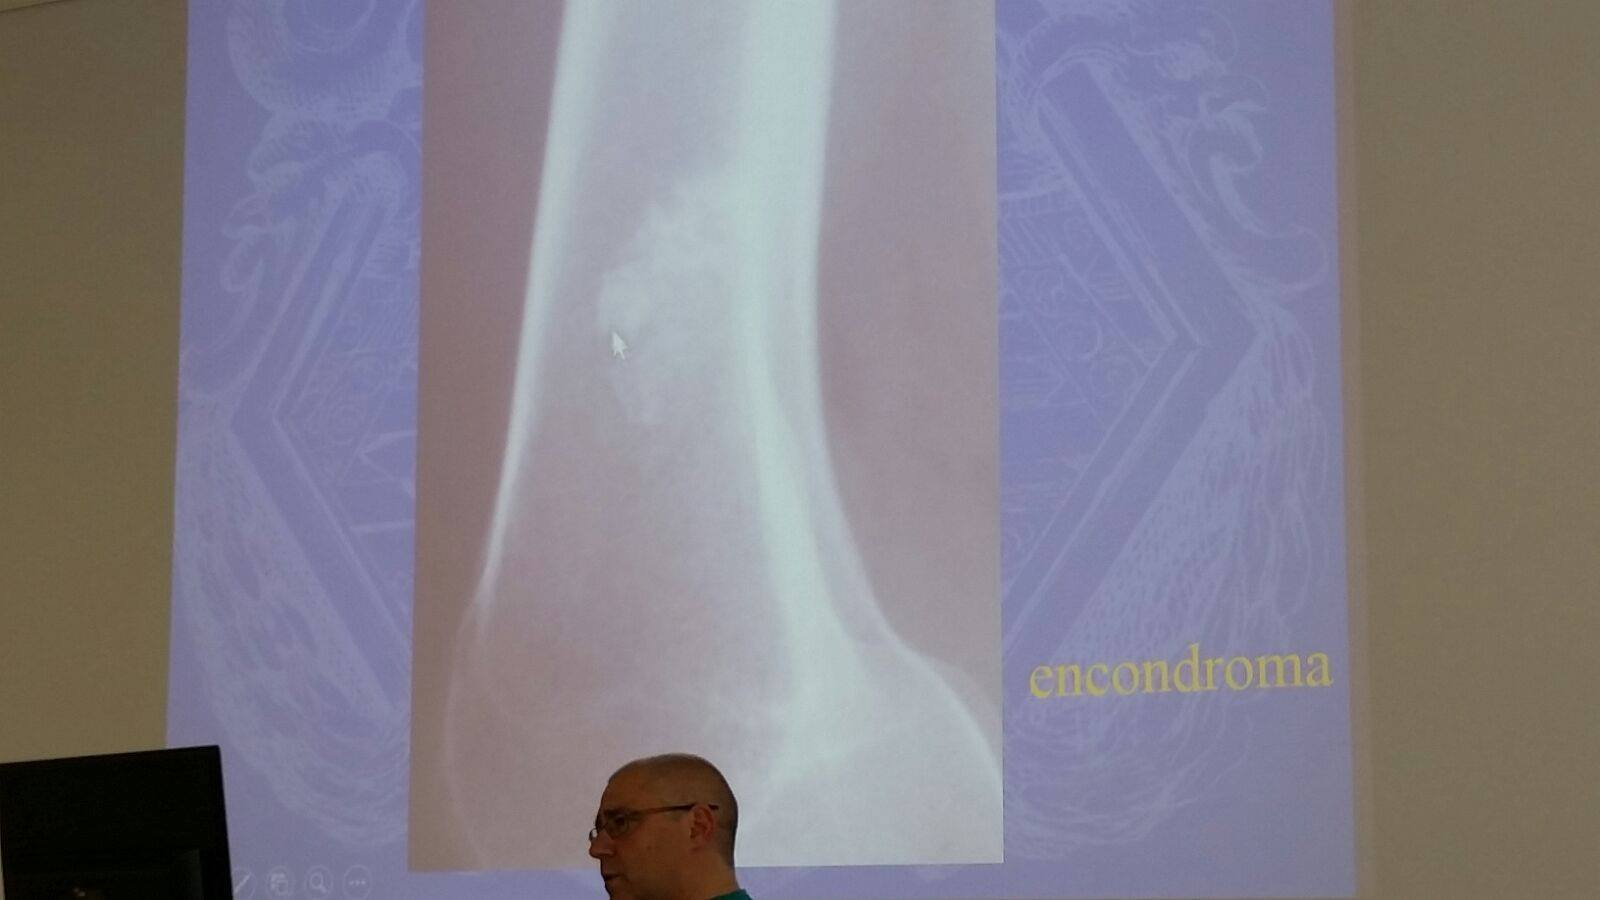
\includegraphics[width=4.93750in,height=3.58333in]{media/image1.jpeg}

Qui vediamo un esempio di encondroma in cui è visibile una zona
punteggiata da piccole calcificazioni all'interno della metafisi distale
del femore. L'aspetto benigno sta nel fatto che è localizzata
all'interno dell'osso, le corticali sono indenni, non c'è stata
espansione e non ci sono dei segni nella zona periostale attorno alla
corticale ossea (che potrebbero far pensare ad una neoplasia maligna).

Encondroma Multiplo

(malattia di Ollier)

Oltre a singolo l'encondroma può essere \textbf{multiplo} e in questo
caso corrisponde ad una malattia ereditaria che prende il nome di
malattia di Ollier.

Questa forma può avere un'evoluzione maligna e perciò una trasformazione
di questi encondromi benigni in \textbf{condrosarcomi}.

I pazienti che presentano la malattia di Ollier devono quindi essere
seguiti nel tempo per la possibile degenerazione sarcomatosa.

Esostosi

È una \textbf{protrusione} dell'osso ricoperta da cartilagine che può
esistere in forma solitaria o multipla. Generalmente compare tra i 10 e
12 anni di età.

I \textbf{sintomi} sono scarsi, quasi assenti. A volte sono legati alla
sporgenza dell'osso; ad esempio una esostosi a livello della testa del
perone può portare ad una compressione del nervo sciatico esterno e dare
dolore. Le sporgenze possono essere palpate a livello dell'estremità
metafisarie.

Qualora diano fastidio o creino inestetismi si possono rimuovere
\textbf{chirurgicamente} a livello della base. Come prima cosa si
isolano le strutture che passano attorno all'esostosi, poi con una sega,
un colpo di scalpello alla base, l'esostosi viene eliminata.

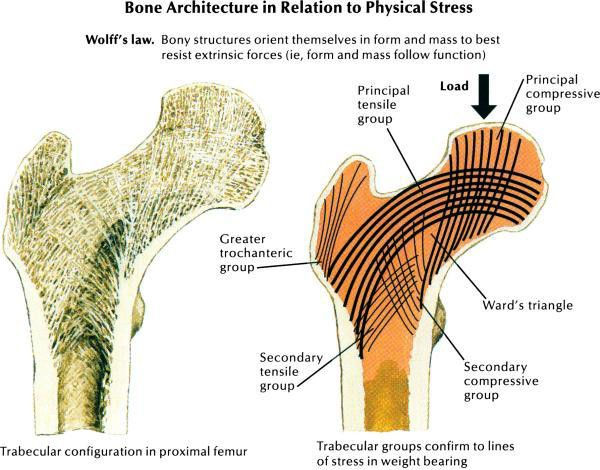
\includegraphics[width=4.39583in,height=3.35417in]{media/image2.jpeg}

In questo caso vediamo una esostosi solitaria a livello della testa del
perone.

\emph{Tumori maligni cartilaginei}

Condrosarcoma

È un tumore particolarmente aggressivo che può portare a metastasi a
distanza.

Può avere una duplice \textbf{origine}:

1. Centrale, più frequentemente. Le cellule maligne cartilaginee
originano all'interno dell'osso, tipicamente nell'aduto.

2. Periferica, più raramente. L'esostosi singola o multipla può andare
incontro ad una trasformazione condrosarcomatosa in forma periferica.

Causa un \textbf{dolore} profondo, sordo, continuo, ma non acuto.
L'evoluzione è lenta.

Il \textbf{trattamento} di solito è chirurgico con un'asportazione della
neoplasia ampia, a volte preceduta, ma soprattutto seguita da
chemioterapia e radioterapia.

Il Prof. mostra un condrosarcoma dell'estremità prossimale del femore in
cui si vede una lisi quasi sepimentata con delle calcificazioni
all'interno della struttura ossea. Vi è interessamento calcifico dei
tessuti molli periarticolari.

Oltre alla clinica, alla \textbf{radiografia} e alla \textbf{risonanza
magnetica} con mezzo di contrasto si fa riferimento
all'\textbf{istologia} (anche quella intraoperatoria a freddo) per
determinare la natura e la malignità della neoplasia.

\emph{Altri tumori}

Tumore Gigantocellulare

Tumore abbastanza frequente, può colpire l'osso ma anche le strutture
molli (es. guaine dei tendini a livello della mano).

È caratterizzato da un accumulo di cellule giganti, lo ritroviamo
generalmente negli adulti in sede \textbf{epifisaria}.

A differenza del condrosarcoma questo tumore da una lisi moltiloculata
dell'osso interessato senza reazione periostale.

Viene utilizzato un \textbf{trattamento} chirurgico, bisogna esportare
la massa, pulire bene il tutto perché le possibilità di recidive
esistono in maniera importante.

È un tumore benigno a grossa \textbf{invasività} locale.

Sarcoma di Ewing

Tumore molto aggressivo, maligno, generalmente di età adolescenziale che
a differenza dell'osteosarcoma e condrosarcoma tende a colpire la
\textbf{diafisi} delle ossa lunghe.

Può essere associato a febbre e malessere.

È necessario fare diagnosi differenziale con l'osteomielite acuta
ematogena.

La \textbf{terapia} è una chemioterapia preoperatoria anche in questo
caso associata ad una chirurgia abbastanza aggressiva con una resezione
ampia.

Tipica è la reazione periostale a bulbo di cipolla dal punto di vista
radiografico e della risonanza magnetica (è una reazione della corticale
che si ispessisce e dà questo aspetto).

\emph{Tumori Metastatici}

Tumori anche più frequenti delle neoplasie primitive.

Sono per definizione la localizzazione secondaria di un tumore
primitivo.

Possono esistere diverse \textbf{forme}:

\begin{itemize}
\item
  \emph{\textbf{forme litiche}}: tipico del carcinoma della tiroide, del
  colon retto, renale associate ad un aumento della calcemia e ad un
  eccessiva calciuria e idrossiprolinuria.
\item
  \emph{\textbf{forme osteoaddensanti}}: tipiche invece del carcinoma
  della prostata e caratterizzate da un aumento della fosfatasi
  alcalina.
\item
  \emph{\textbf{forme miste}}: determinate a livello osseo dal carcinoma
  della mammella. Sono forme osteolitiche e addensanti.
\end{itemize}

Anche in questo caso il \textbf{dolore} è cronico, sordo, continuo, non
acuto.

A volte si estrinsecano con una frattura patologica.

Trattamento

La \textbf{terapia} solitamente è multidisciplinare.

In linea di massima, se la metastasi è unica con una buona prognosi quod
vitam si può fare un trattamento di \textbf{eradicazione}, ossia
un'asportazione della metastasi e sostituzione del segmento osseo che è
stato metastatizzato con una protesi.

Se le metastasi sono multiple con prognosi quod vitam non
particolarmente alta allora non si fanno eradicazioni, ma si possono
fare degli \textbf{inchiodamenti preventivi} per evitare fratture
patologiche e ci si affida ad una radioterapia o chemioterapica
associata.

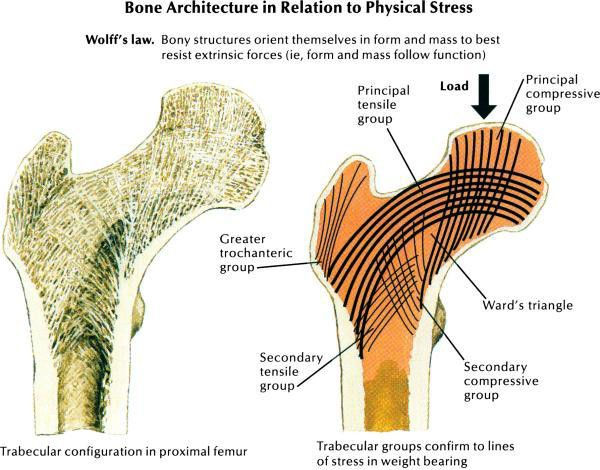
\includegraphics[width=4.88542in,height=3.82292in]{media/image3.jpeg}

Carcinoma prostatico con metastasi osteoaddensante in corrispondenza di
una vertebra cervicale bassa.

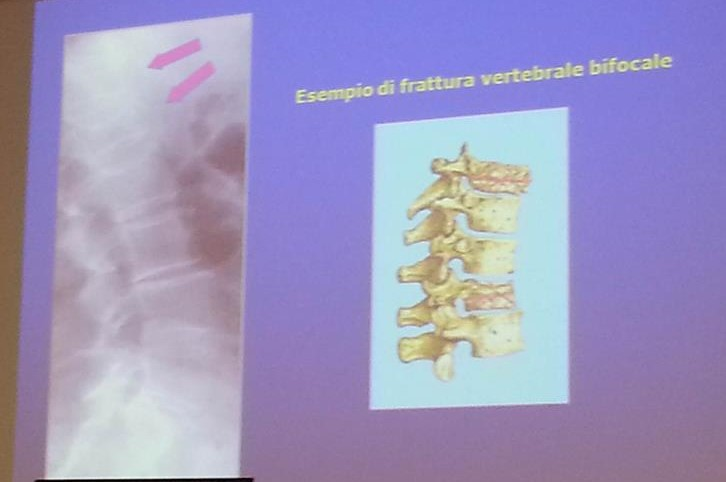
\includegraphics[width=5.15625in,height=4.14583in]{media/image4.jpeg}

Carcinoma renale con osteolisi a tutto il bacino e zona trocanterica:
metastasi osteolitica.

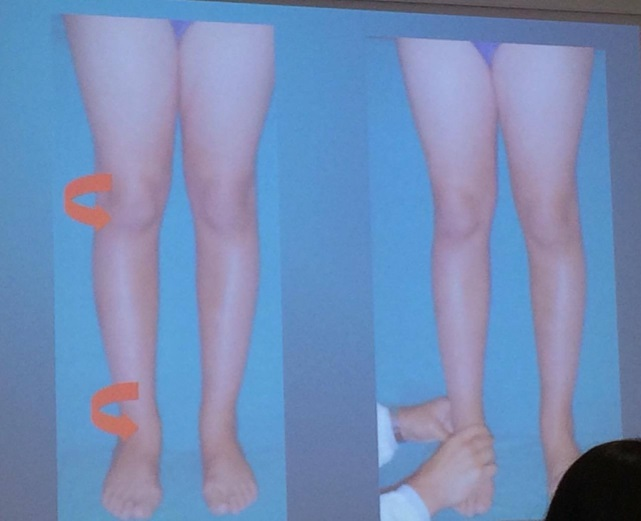
\includegraphics[width=4.97917in,height=4.01042in]{media/image5.jpeg}

Carcinoma mammario misto addensante osteolitico, addensante osteolitico.